\documentclass[12pt,a4paper,titlepage]{scrartcl}
%evtl. nützliche Pakete
\usepackage[utf8]{inputenc}
\usepackage[ngerman]{babel}
\usepackage{oldgerm}
\usepackage[top=3.0cm,right=2.0cm,bottom=3.0cm,left=2.0cm]{geometry}
\usepackage{amsmath}
\usepackage{amssymb}
\usepackage{stmaryrd}
\usepackage[right]{eurosym} %mit `\euro' oder `\euro{Betrag}' zu benutzen
\usepackage{listings}
\usepackage{mdwlist} %ermöglicht mit z.B. itemize* den Zeilenabstand in Aufzählungen kleiner zu machen
\usepackage{fancyhdr}
\usepackage{graphicx}
\usepackage{hyperref} %verlinkt automatisch alle Referenzen, sodass am Rechner mit Mausklicken dort hin gesprungen wird.
\usepackage{pdfpages}

%Abkürzungen langer Befehle
\renewcommand \( {\left (}
\renewcommand \) {\right )}
\renewcommand \[ {\left [}
\renewcommand \] {\right ]}
\newcommand \Flqq {\flqq\ }
\newcommand{\lola}{\frqq LoLA\Flqq}


%Sonstiges
\parindent 1.0cm
\subject{\lola}
\title{Anleitung zur Erstellung eines neuen Stores}
\author{Max Görner}
\publishers{Betreuer:\\ Prof. Dr. rer. nat Karsten Wolf\\ Dr. ing. Niels Lohmann}
\date{\today}


\lstset{language=C++}
\begin{document}
\maketitle
%\tableofcontents
Im Rahmen dieser Anleitung soll erläutert werden, wie für das Petrinetzanalyseprogramm \lola ein neuer Store geschrieben werden kann. Dafür wird zunächst behandelt, was ein Store ist und wie ein Store strukturiert ist. Danach wird erklärt, wie ein neuer Store etabliert werden kann. Da fast alle Stores PluginStores sind, werden diese sowie deren Komponenten, NetStateEncoder und VectorStores, im Anschluss vorgestellt.

\section{Allgemeine Stores}
Um Petrinetze zu analysieren, müssen im Wesentlichen alle erreichbaren Netzzustände (sog. NetStates
\footnote{Ein NetState ist eine Klasse, die sowohl die Anzahl der Markierungen auf jeder Stelle, als auch zusätzliche, zur Beschleunigung des Programmes dienende Informationen enthält. In Stores werden jedoch nur die Markierungsanzahlen gespeichert.}
) einmal besucht werden. Daher wird eine Datenstruktur benötigt, die es ermöglicht, für einen übergebenen NetState zu bestimmen, ob dieser vorher schon einmal übergeben wurde und sich diesen danach zu merken.

Stores bieten eine solche Datenstruktur über eine einheitliche Schnittstelle an. Dafür muss jeder Store von der Klasse \frqq Store
\footnote{Die Oberklasse aller Stores ist in \frqq src/Stores/Store.h\Flqq definiert.}
\Flqq erben und folgende Funktionen implementieren:
\begin{description}
\item[get\_number\_of\_calls] Diese Funktion gibt die Anzahl der Aufrufe der Funktion \frqq searchAndInsert\Flqq zurück.
\item[get\_number\_of\_markings] Diese Funktion gibt die Anzahl der gespeicherten NetStates zurück. Diese wird neben anderen Zwecken zur Fehlersuche und zur Angabe der Programmgeschwindigkeit benötigt.
\item[popState] Diese Funktion entfernt eine Markierung aus dem Store und gibt sie zurück.
\item[searchAndInsert] Diese Funktion nimmt einen Zustand des Petrinetzes entgegen und speichert diesen gegebenenfalls. Außerdem gibt sie zurück, ob dieser Zustand schon früher übergeben wurde und reserviert gegebenenfalls Speicherplatz für Zusatzinformationen (sog. Payload). Diese Funktion ist eine der kritischsten Stellen des gesamten Programmes, da hier große Teile der Laufzeit verbraucht werden. Es ist daher erwünscht, dass diese Funktion threadsicher implementiert wird, um Nutzen aus Parallelisierungen ziehen zu können.
\end{description}
Weiterführende Details können den Kommentaren des Quellcodes oder der daraus abgeleiteten Doxygendokumentation entnommen werden.

\section{PluginStores
\protect\footnote{Die Oberklasse aller PluginStores ist in \frqq src/Stores/PluginStore.h\Flqq definiert.}}
\label{kap:PluginStores}
Es gibt sowohl für die Kodierung der NetStates, als auch für die verwendete Datenstruktur mehrere Alternativen, die sich in verschiedenen Kontexten anbieten. So könnte bei sehr speicherplatzintensiven Petrinetzen eine Komprimierung der NetStates erwünscht und der damit verbundene Geschwindigkeitsverlust hinnehmbar sein, während in anderen Fällen auf schnellstmögliche Ausführungsgeschwindigkeit gewünscht ist. Um nun die Vor- und Nachteile der verschiedenen Kodierungen und Datenstrukturen möglichst einfach kombinieren zu können, wurde das Konzept der PluginStores entworfen.

Ein \frqq PluginStore\Flqq ist ein Store, der den oben umrissenen Bedingungen genügt. Allerdings verwendet er einen NetStateEncoder, um die NetStates wie gewünscht zu kodieren, und einen VectorStore, um Bitvektoren, das Resultat der Kodierung eines NetStates durch einen NetStateEncoder, abzuspeichern und wiederzufinden. Dadurch können prinzipiell alle Kodierungen mit allen Datenstrukturen kombiniert werden. Einzelne Komponennten können jedoch in ihrem Funktionsumfang eingeschränkt sein. Abbildung \ref{fig:plugin} verdeutlicht das Prinzip der PluginStores.
\begin{figure}[ht]
	\begin{center}
		%TODO: Grafik verbessern: Im ersten Oval müsste die Funktion stehen, die einen NetState an den PluginStore sendet. Schon "LoLA wäre passender als "NetState".
		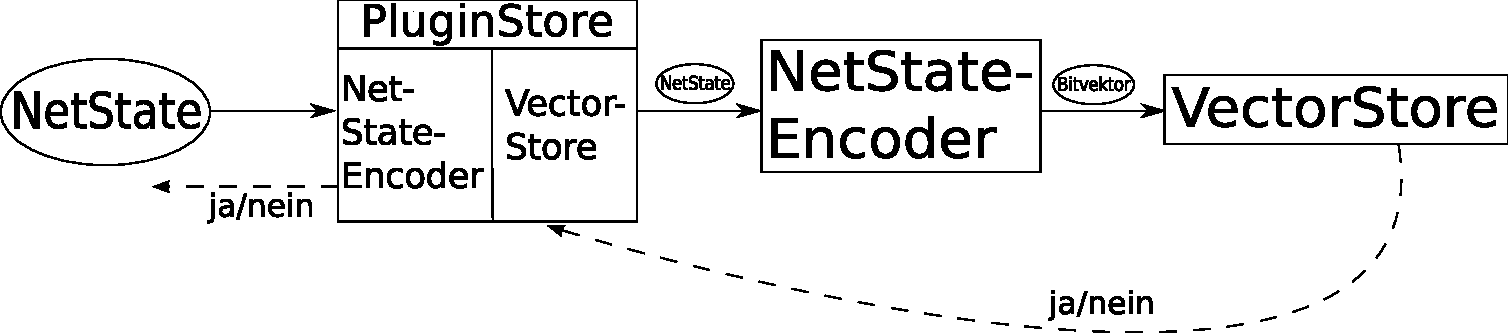
\includegraphics[width = 0.9\textwidth]{Schema.pdf}
		\caption{Diese Grafik zeigt den Ablauf der Verarbeitung eines Aufrufes der Funktion \frqq searchAndInsert\flqq .}
		\label{fig:plugin}
	\end{center}
\end{figure}

Im folgenden soll erläutert werden, wie ein neuer NetStateEncoder und ein neuer VectorStore geschrieben werden können.


\subsection{NetStateEncoder
\protect\footnote{Die Oberklasse aller NetStateEncoder ist in \frqq src/Stores/NetStateEncoder/NetStateEncoder.h\Flqq definiert.}}
\label{kap:NetStateEncoder}
Ein NetStateEncoder (NSE) bildet einen NetState auf Bitvektor ab, damit dieser von einem VectorStore gespeichert werden kann. Die Länge der Bitvektoren muss hierbei keineswegs konstant sein.

Ziel der Abbildungen ist es, die unterschiedlichen Abwägungen verschiedener Einsatzgebiete zu Speicherverbrauch und Laufzeit zu berücksichtigen. Es gibt bisher folgende NSE:
\begin{description}
\item[FullCopyEncoder] Dieser NSE kopiert alle Stellen eines NetStates.
\item[CopyEncoder] Dieser NSE kopiert nur die signifikanten Stellen eines NetStates und verwirft damit jene, die sich aus Stelleninvarianten ergeben. Dies kann Speicherplatz sparen, erschwert dann aber die Rekonstruktion des vollständigen NetStates.
\item[BitEncoder] Der BitEncoder arbeitet prinzipiell wie der CopyEncoder. Sollte für die Anzahl der Marken auf den Stellen des zu untersuchenden Petrinetzes eine obere Schranke $s$ angegeben worden sein, verwendet es nur $\lceil \log_2(s)\rceil$ viele Bits zur Kodierung der Markenanzahl. Bei Netzen mit kleiner oberer Schranke ergeben sich dadurch sehr hohe Kompressionsgrade.
\item[SimpleCompressedEncoder] Dieser NSE kodiert die einzelnen Stellen mit logarithmischer Länge und nutzt damit aus, dass kleine Zahlen besonders häufig vorkommen. Dies reduziert den Speicherverbrauch um einen Divisor bis zu $10$, verlängert aber auch die Laufzeit erheblich.
\end{description}
Die genauen Geschwindigkeitseinbußen und Speicherplatzgewinne hängen von der konkreten Struktur des untersuchten Petrinetzes ab.

Ein NetStateEncoder muss die Funktion \frqq\textbf{encodeNetState}\Flqq bereitstellen, welche einen übergebenen NetState auf einen Bitvektor abbildet und diesen zurück gibt.

Ein NetStateEncoder kann die Funktion \frqq\textbf{decodeNetState}\Flqq bereitstellen, welche die Umkehrfunktion zur Abbildungsfunktion \frqq encodeNetState\Flqq darstellt. Sie übernimmt damit einen Bitvektor und gibt einen NetState zurück.

Weiterführende Details können den Kommentaren des Quellcodes oder der daraus abgeleiteten Doxygendokumentation entnommen werden.

Damit ein neu geschriebener NetStateEncoder kompiliert wird, müssen seine Quellcodedateien in die Liste \frqq lola\_SOURCES\Flqq in der Datei \frqq src/Makefile.am\Flqq eingetragen werden.

\subsection{VectorStores
\protect\footnote{Die Oberklasse aller VectorStores ist in \frqq src/Stores/VectorStores/VectorStore.h\Flqq definiert.}}
\label{kap:VectorStores}
Ein VectorStore ist kein Store im oben beschriebenen Sinne, da VectorStores nicht von der Klasse Store erben. Ansonsten ähnelt die Funktionsweise von VectorStores der von Stores.

Der wesentliche Unterschied besteht darin, dass VectorStores nicht NetStates, sondern von NetStateEncodern als Bitvektoren kodierte NetStates speichern. Außerdem kümmern sie sich nicht um die Zählung von Aufrufen und Markierungen. Damit gibt es folgende Funktionen:
\begin{description}
\item[popVector] Diese Funktion entfernt einen von NetStateEncodern als Bitvektoren kodierten NetState aus dem VectorStore und gibt ihn zurück. 
\item[searchAndInsert] Diese Funktion nimmt einen Bitvektor entgegen und speichert diesen gegebenenfalls. Außerdem gibt sie zurück, ob dieser Bitvektor schon früher übergeben wurde und reserviert gegebenenfalls Speicherplatz für Zusatzinformationen (sog. Payload). Wie bei Stores ist diese Funktion die geschwindigkeitskritischste Funktion im gesamten Programm und sollte daher threadsicher sein.
\end{description}
Die Konzentration auf Bitvektoren ist wichtig, um Speicherplatz sparen zu können. Die Funktion \frqq searchAndInsert\Flqq nimmt dafür einen Zeiger und eine Länge in Bits entgegen. Nun können Datenstrukturen entwickelt und verwendet werden, die bitexakt arbeiten.

Ein leicht verständliches Beispiel für eine solche Datenstruktur ist eine Liste. Werden Listen als großer zu\-sammen\-hängen\-der Speicherbereich implementiert, in den die Elemente hintereinander geschrieben werden, ist es ohne weiteres möglich, Bitvektoren direkt hintereinander zu schreiben. Damit beträgt der größtmögliche Verschnitt 7 Bit und ist vernachlässigbar.

Folgende VectorStores existieren bisher:
\begin{description}
\item[BloomStore] Dieser VectorStore basiert auf Hashfunktionen. Dadurch verbraucht er sehr wenig Speicher, kann aber falsche Antworten geben.
\item[CompareStore] Dieser VectorStore vergleicht die Ergebnisse zweier Stores. Damit können neue Stores einfach auf Korrektheit getestet werden. Auf diesen Store wird in Kapitel \ref{kap:CompareStore} näher eingegangen.
\item[PrefixTreeStore:] Dieser VectorStore kann Vektoren ohne Verschnitt speichern. Er ist sehr schnell und speichereffizient. Er verwendet Präfixbäume als Datenstruktur.
\item[SuffixTreeStore:] Dieser VectorStore kann Vektoren ohne Verschnitt speichern. Er ist sehr schnell und speichereffizient. Er verwendet Präfixbäume als Datenstruktur.
\item[VSTLStore:] Dieser VectorStore verdeutlicht das Prinzip von Stores. Sein didaktischer Nutzen ist größer als der für den produktiven Einsatz. Er verwendet als Datenstruktur STL-Sets, in denen STL-Vektoren gespeichert werden.
\end{description}

Weiterführende Details können den Kommentaren des Quellcodes oder der daraus abgeleiteten Doxygendokumentation entnommen werden.

Damit ein neu geschriebener VectorStore kompiliert wird, müssen seine Quellcodedateien in die Liste \frqq lola\_SOURCES\Flqq in der Datei \frqq src/Makefile.am\Flqq eingetragen werden.

\subsection{Verwendung von PluginStores}
Wenn der gewünschte NetStateEncoder und VectorStore vorhanden sind, müssen für die Erstellung eines neuen PluginStores keine neuen Dateien angelegt werden. Es reicht, eine neue Klasse zu erstellen und einer entsprechenden Variablen zuzuweisen. Beispiele finden sich in Listing \ref{lst:PluginStore} und in der Datei \frqq src/Planning/Tasks.h\Flqq.

\section{Templates und Payload}
Diverse Algorithmen von \lola erfordern es, NetStates nicht nur zu speichern, sondern zu diesen auch Zusatzinformationen, sogenannte Payloads, hinterlegen zu können. Aus diesem Grund verwenden alle Stores Templates. Diese ermöglichen es, dass jede Art Payload, von primitiven Datentypen bis hin zu ganzen Klassen, hinterlegt werden kann. Dieses Kapitel beschreibt die bisherigen Konventionen, die eingehalten werden sollten.

Die Verwendung von Templates beschränkt sich momentan darauf, die Signaturen der betroffenen Funktionen, sowie die Art gewisser Variablen und Rückgabetypen variabel zu halten. Bis auf eine Ausnahme,
\frqq Store$<$void$>$\Flqq verändern Templates momentan nicht die Arbeitsweise der Stores.

Damit im Falle des Verzichts auf Payload kein Speicherplatz verschwendet wird, wurde \frqq void\Flqq als Schlüsselwort dafür definiert, dass kein Payload hinterlegt werden wird. Dementsprechend wird im Listing \ref{lst:PluginStore}

\begin{center}
\begin{minipage}{0.7\textwidth}
\lstset{language=C++}
\begin{lstlisting}[label=lst:PluginStore,caption={Erstellung eines PluginStores}]
s = new PluginStore<void>(
   new SimpleCompressedEncoder(number_of_threads),
   new SuffixTreeStore<void>(), number_of_threads);\end{lstlisting}
\end{minipage}
\end{center}
%
der Variablen s ein PluginStore, der intern einen SuffixTreeStore verwendet, aber keinerlei Speicherplatz für Payload verbraucht, zugewiesen. Es wird nicht einmal Speicherplatz für Variablen verbraucht, die nur für die Verwaltung des Payload interessant wären.

Durch die Verwendung von Templates ist es in den betroffenen Klassen nicht möglich, die übliche Aufteilung in einen Definitionsteil (.h-Datei) und einen Implementierungsteil (.cc-Datei), wobei die .h-Datei in der .cc-Datei inkludiert wird, beizubehalten. Eine ausführliche Erklärung dazu findet sich im Buch \frqq C++ Templates: The Complete Guide\Flqq von Josuttis und Vandevoorde. Um trotzdem eine ähnliche Struktur beibehalten zu können, gibt es eine kurze und übersichtliche Datei mit Definitionen (.h-Datei), sowie einer Datei mit den Implementierungen (.inc-Datei), wobei am Ende der ersten die zweite inkludiert wird. Dies entspricht dem \frqq Inclusion Model\Flqq aus dem genannten Buch.

\subsection{Bucketing}
Ein weiterer, besonderer VectorStore ist der \frqq HashingWrapperStore\flqq\footnote{Der HashingWrapperStore ist in der Datei \frqq src/Stores/VectorStores/HashingWrapperStore.h\Flqq definiert.}. Dieser verwaltet intern sehr viele VectorStores und versucht die zu speichernden NetStates auf diesen möglichst gleichmäßig zu verteilen. In diesem Abschnitt werden zunächst die Vor- und Nachteile dieser Technik erläutert. Im Anschluss wird erläutert, wie Bucketing bei der Erstellung neuer Stores genutzt werden kann.

\subsubsection{Vor- und Nachteile}
Bei allen Stores außer dem BloomStore hängt die Zeit für einen Aufruf der Funktion \frqq searchAndInsert\Flqq logarithmisch von der Anzahl der gespeicherten NetStates ab. Diese Anzahl wird oft sehr groß. Eine Beschleunigung\footnote{Diese Beschleunigung ändert nicht die asymptotische Komplexität sondern beschleunigt um einen konstanten Faktor.} mit nur konstantem Speichermehrverbrauch kann daher erreicht werden, wenn die Markierungen durch geeignete Hashfunktionen sehr schnell auf viele verschiedene Stores aufgeteilt werden können, da die Anzahl der gespeicherten Netzzustände pro Store damit stark reduziert wird. Diese Aufteilung übernimmt der HashingWrapperStore.

Zusätzlich zur direkten Beschleunigung ist der HashingWrapperStore auch eine einfache Variante, mit beliebigen VectorStores eine Parallelisierung zu erreichen, da die einzelnen Stores voneinander unabhängig sind.

Allerdings wird bei der Verwendung des HashingWrapperStores mehr Arbeitsspeicher verbraucht. Schon die Erstellung und Vorhaltung sehr vieler Stores verbraucht etwas Speicherplatz. Dieser nur konstante Mehrverbrauch dürfte jedoch in den meisten Fällen vernachlässigbar sein. Viel gewichtiger ist, dass einige Stores, momentan der PrefixTreeStore und SuffixTreeStore, die Netzzustände speicherschonend abspeichern. Bei den beiden genannten Stores werden beispielsweise gleiche Anfänge in der Bitdarstellung zweier Vektoren nur genau ein Mal gespeichert. Diese Einsparung ist nicht mehr möglich, wenn Vektoren mit gleichen Anfangsstücken in unterschiedlichen Buckets landen.

\subsubsection{Verwendung des Bucketing}
Bucketing wird durch den Parameter \frqq --bucketing\Flqq angestellt. Wie selbstgeschriebene Stores in \lola integriert werden, wird im Kapitel \ref{kap:Etablierung} erläutert. Hier wird erläutert, wie die Erstellung von HashingWrapperStores funktioniert.

Ein HashingWrapperStore ist ein auf Templates basierender Store, dessen Konstruktor einen VectorStoreCreator\footnote{Die Definition findet sich in der Datei des HashingWrapperStores.} (VSC) entgegennimmnt. Ein VSC wird benötigt, da eine variable Anzahl Stores erstellt werden muss. Es genügt daher nicht, den gewünschten Store zu übergeben; vielmehr wird eine beliebig oft aufrufbare Funktion benötigt, die den gewünschten Store übergibt. VSC übernehmen genau diese Aufgabe.

Da die Konstruktoren verschiedener Stores eine unterschiedliche Anzahl von Parametern erwarten, gibt es verschiedene VSC, namentlich den \frqq NullaryVectorStoreCreator\frqq, den \frqq UnaryVectorStoreCreator\Frqq sowie den \frqq BinaryVectorStoreCreator\flqq\footnote{Alle definiert in der Datei des HashingWrapperStores.}, die VectorStores mit keinem bis zwei Parametern erstellen. Eine Unterstützung weiterer Parameteranzahlen ist denkbar, aber bis jetzt nicht notwendig gewesen. Mit dem schon vorhandenen Quellcode sollten weitere VSC einfach implementiert werden können.

Ein konkretes Beispiel zur Erstellung eines PluginStores mit Bucketing ist in Listing \ref{lst:HashingWrapperStore} zu sehen.

\begin{center}
\begin{minipage}{0.7\textwidth}
\lstset{language=C++}
\begin{lstlisting}[label=lst:HashingWrapperStore,caption={Erstellung eines PluginStores mit Bucketing. Dem HashingWrapperStore wird ein UnaryVectorStoreCreator übergeben, welcher einen VSTLStore erstellt. Das Argument des VSC-Konstruktors wird an jeden erstellten VSTL-Store weitergereicht.}]
s = new PluginStore<T>(
	new BitEncoder(number_of_threads),
	new HashingWrapperStore<T>(
		new UnaryVectorStoreCreator
			<T,VSTLStore<T>,index_t>
			(number_of_threads)
		),
	number_of_threads);
\end{lstlisting}
\end{minipage}
\end{center}


\section{Etablierung eines neuen Stores}
\label{kap:Etablierung}
Um einen neu geschriebenen Store verwenden zu können, müssen für diesen neue Kommandozeilenparameter eingeführt werden. Außerdem muss der Store in den Kompilierungsprozess und die Korrektheitstest integriert werden.

\subsection{Kommandozeilenparameter einführen}
Neue Kommandozeilenparameter werden auf einfache Weise in der Datei \frqq cmdline.ggo\Flqq angegeben.

Soll ein Parameter für einen neuen Store erstellt werden, muss für diesen ein Parameter in der Rubrik \frqq stores\Flqq hinzugefügt werden.

Soll ein Parameter für einen neuen NetStateEncoder erstellt werden, muss für diesen ein Parameter in der Rubrik \frqq encoder\Flqq hinzugefügt werden.

Um mit den so definierten Kommandozeilenparametern die neuen NetStateEncoder aufrufen zu können, mussen in der Klasse \frqq StoreCreator\Flqq in den Dateien \frqq src/Planning/Tasks.h\Flqq und \frqq src/Planning/Tasks.cc\Flqq die Funktion \frqq createStore()\Flqq angepasst werden. Dies geschieht, indem in beiden Dateien der entsprechende switch-case-Block erweitert wird. Der anzugebende case-Schlüssel besteht hierbei aus dem Präfix \frqq encoder\_arg\_\Flqq und dem in der Datei \frqq cmdline.ggo\Flqq eingetragenen Parameter.

Um neue Stores mit Payload-Informationen verwenden zu können, muss der entsprechende switch-case-Block in der Task.h erweitert werden. Der anzugebende case-Schlüssel besteht hierbei aus dem Präfix \frqq store\_arg\_\Flqq und dem in der Datei \frqq cmdline.ggo\Flqq eingetragenen Parameter. Sollte beim neuen Store die Verwendung von Hash-Buckets sinnvoll sein, muss dies innerhalb des case-Blocks unterschieden werden. Dies kann durch Abfrage, ob die Variable \frqq args\_info.bucketing\_given\Flqq gesetzt ist, herausgefunden werden. Um dann einen Hash-Buckets verwendenden Store zu erstellen, muss dem PluginStore als VectorStore ein HashingWrapperStore übergeben werden.

%Vorgehen mit createSpecializedStore erklären

\subsection{Kompilierungsprozess erweitern}
Damit ein neu geschriebener Store oder NetStateEncoder kompiliert wird, müssen die entsprechenden Quellcodedateien in die Liste \frqq lola\_SOURCES\Flqq in der Datei \frqq src/Makefile.am\Flqq eingetragen werden.

\subsection{Korrektheitstest}
Gerade bei der Entwicklung neuer Funktionen können Fehler gemacht oder entdeckt werden. Daher bietet \lola eine Reihe von Maßnahmen, diese z finden. In diesem Abschnitt werden die auf Stores bezogenen Qualitätssicherungsmaßnahmen behandelt.

\subsubsection{Der CompareStore}
\label{kap:CompareStore}
Gerade bei der Entwicklung neuer Stores ist nicht immer ganz klar, ob diese Stores alle Netzzustände zuverlässig speichern und wiederfinden. Dies überprüft der CompareStore, indem er die Rückgaben zweier Stores vergleicht. Sind diese unterschiedlich, beendet sich das Programm.

Um einen zu überprüfenden Store anzugeben, muss dieser in der Task.h anstelle eines der momentan dort als Parameter des CompareStores eingetragenen Stores angegeben werden.

\subsubsection{Automatisierte Korrektheitstests}
In \lola wurden einige Korrektheitstest automatisiert. Es gibt Tests, die prüfen, ob \lola unter Verwendung der zu testenden Stores das erwartete Ergebnis berechnet. Es gibt ähnliche Tests, die dafür jedoch mehrere Threads verwenden und somit Fehler im Threading feststellen können. Abschließend gibt es noch Tests, die überprüfen, ob die Speicherverwaltung der Stores allen angeforderten Speicher wieder frei gibt.

Um einen Store in einen der oben genannten Tests einzubinden, muss in der Datei
\\\frqq tests/testsuit.at\Flqq in den entsprechenden Bereichen der entsprechende Befehl eingegeben werden.

Die Bereiche sind, entsprechend der obigen Reihenfolge, \frqq AT\_BANNER([Stores])\Flqq,\\\frqq AT\_BANNER([Parallel Stores])\Flqq und \frqq AT\_BANNER([Memory Management])\flqq.

Die Syntax der Befehle ergibt sich aus den schon vorhandenen Befehlen und den Kommentaren in der genannten Datei. Es muss für jedes Netz, mit dem die entsprechende Eigenschaft überprüft werden soll, eine Anweisung erstellt werden.

Im Anschluss können mit \frqq make check\Flqq die automatischen Korrektheitstest gestartet werden, in denen der neu integrierte Store auftauchen sollte.
\end{document}






















